\subsection{Fonctions de parking rationnelles}

Cette partie est illustrée par les exemples 17 à 19 de l'annexe C.

\begin{definition}[a, b - Fonction de Parking]
    Une \emph{a, b - fonction de parking} est une séquence d'entiers
    positifs $(a_1, a_2, \ldots, a_n)$ telle que :\\
    \begin{itemize*}
        \item $n = a$\\
        \item son tri croissant $(b_1, b_2, \ldots, b_n)$ respecte la
        condition suivante :$b_i \leqslant \frac{b}{a}(i-1) + 1$ 
        pour tout $i \leqslant n$.
    \end{itemize*}
\end{definition}

On note $\mathcal{PF}_{a,b}$ l'ensemble des a, b - fonctions de parking. 

\begin{theorem}[Armstrong, Loehr et Warrington, 2014]
    Soit $pf_{a,b}$ le cardinal de $\mathcal{PF}_{a,b}$.
    Nous avons $$pf_{a,b} = b^{a-1}$$
\end{theorem}

\begin{rem}
Le cas classique peut être vu comme le cas $a = n, b = n + 1$.
Autrement dit, $\mathcal{PF}_{n, n + 1} = \mathcal{PF}_n$.
\end{rem}

Similairement au cas classique, on définit une fonction de parking
\emph{rationnelle primitive} comme une fonction de parking primitive
triée en ordre croissant.
On note $\mathcal{PF'}_{a,b}$ l'ensemble des a, b - fonctions de parking
primitives.

\begin{theorem}
    Soit $pf'_{a,b}$ le cardinal de $\mathcal{PF'}_{a,b}$.
    Nous avons $$\displaystyle pf'_{a,b} = 
    \frac{1}{a + b} \binom{a + b}{b}$$
\end{theorem}

Ce nombre est appelé le \emph{nombre de Catalan rationnel}, et on le note
$Cat(a,b)$.
Là aussi, le cas classique correspond à $a = n, b = n + 1$.
Autrement dit, $\mathcal{PF'}_{n, n + 1} = \mathcal{PF'}_n$.

\subsection{Chemins de Dyck rationnels}

Cette partie est illustrée par les exemples 20 à 25 de l'annexe C.

\begin{definition}[a, b - mot de Dyck]
    Un \emph{a, b - mot de Dyck} est un mot $w \in \{0,1\}^*$ tel que :
    \begin{itemize}
        \item pour tout \emph{suffixe} $w'$ de $w$,
            $\displaystyle |w'|_1 \geqslant \frac{a}{b}|w'|_0$.
        \item $|w|_0 = b$.
        \item $|w|_1 = a$.
    \end{itemize}
\end{definition}

Un a, b - mot de Dyck peut être représenté par un chemin allant du point
$(0,0)$ au point $(b,a)$, et restant au dessus de l'axe $y = \frac{a}{b}x$,
appelé \emph{a, b - chemin de Dyck} :
\begin{itemize}
    \item Chaque $1$ correspond à un \emph{pas Nord} $\uparrow$. 
    \item Chaque $0$ correspond à un \emph{pas Est} $\rightarrow$.
\end{itemize}

On note $\mathcal{R}_{a, b}$ l'ensemble des a, b - mots de Dyck.

\begin{theorem}[Bizley, 1954]
    Soit $r_{a,b}$ le cardinal de $\mathcal{R}_{a,b}$.
    Nous avons $$r_{a,b} = \frac{1}{a+b} \binom {a+b}{a} =
    \frac{(a+b-1)!}{a!b!}$$
\end{theorem}

On remarque ainsi que l'on pourra bien créer une bijection entre
$\mathcal{PF'}_{a,b}$ et $\mathcal{R}_{a,b}$.
Cette bijection sera exactement la même que celle entre $\mathcal{PF'}_n$
et $\mathcal{D}_{n}$.

Il reste maintenant à définir les chemins de Dyck qui seront en bijection
avec $\mathcal{PF}_{a,b}$.

\begin{definition}[a, b - mot de Dyck décoré]
    Un \emph{a, b - chemin de Dyck décoré} est un mot $w \in 
    \{0, \ldots, n\}^*$ tel que :
    \begin{itemize}
        \item pour tout suffixe $w'$ de $w$,
            $\displaystyle|w'|_{\neq 0} \geqslant \frac{a}{b}|w'|_0$.
        \item $|w|_0 = b$.
        \item $|w|_{\neq 0} = a$.
        \item pour tout $i \in \{1, \ldots, a\}$, $w$ a exactement une
            occurence de $i$.
        \item si $w_i \neq 0$ et $w_{i+1} \neq 0$,
            alors $w_i < w_{i+1}$. Autrement dit, les labels des pas Nord
            consécutifs sont croissants.
    \end{itemize}
\end{definition}

Un a, b - mot de Dyck décoré peut être représenté par un chemin allant du
point $(0,0)$ au point $(b,a)$, où chaque pas Nord a un label :
\begin{itemize}
    \item Chaque $i \neq 0$ corresponds à un \emph{pas Nord} $\uparrow$
    dont le label est $i$.
    \item Chaque $0$ correspond à un \emph{pas Est} $\rightarrow$.
\end{itemize}

Ces chemins sont appelés \emph{a, b - chemins de Dyck décorés}.\\
On note $\mathcal{LR}_{a,b}$ l'ensemble des a, b - chemins de Dyck.

\begin{theorem}
    Soit $lr_{a,b}$ le cardinal de $\mathcal{LR}_{a,b}$.
    Nous avons $$lr_{a,b} = b^{a - 1}$$.
\end{theorem}

On retrouve bien le même cardinal que pour $\mathcal{PF}_{a,b}$.
A nouveau, la bijection entre $\mathcal{PF}_{a,b}$ et $\mathcal{LR}_{a,b}$
sera exactement la même que celle entre $\mathcal{PF}_n$ et
$\mathcal{LD}_{n}$.

Les relations de couverture restent inchangées :
\begin{itemize}
    \item Pour $\mathcal{PF'}_{a,b}$ et $\mathcal{PF}_{a,b}$ : $\gtrdot$
    \item Pour $\mathcal{R}_{a,b}$ : $\gtrdot_r = \gtrdot_d$
    \item Pour $\mathcal{LR}_{a,b}$ : $\gtrdot_{lr} = \gtrdot_{ld}$ 
\end{itemize}

On peut maintenant construire nos posets pour le cas rationnel.

\subsection{Posets rationnels}

\begin{expl}[$a > b$ : Les posets de $\mathcal{R}_{5,3}$ et
    $\mathcal{PF'}_{5,3}$]
    ~\\
    \begin{center}
        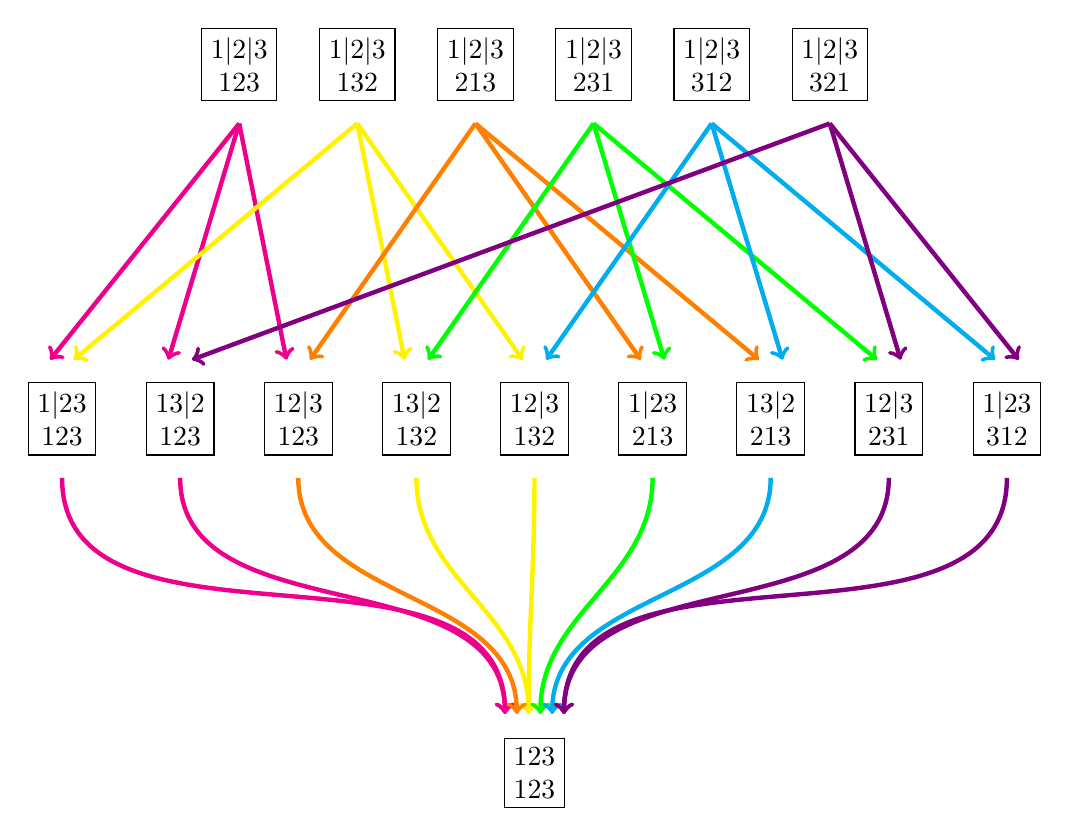
\begin{tikzpicture}[scale = 0.75]
    \node (0)  at (0,0) [align = center]
    [rectangle, draw]
        {$123$\\$123$};
    \node (1)  at (-8,6)[align = center]
    [rectangle, draw]
        {$1|23$\\$123$};
    \node (2)  at (-6,6) [align = center]
    [rectangle, draw]
        {$13|2$\\$123$};
    \node (3)  at (-4,6) [align = center]
    [rectangle, draw]
        {$12|3$\\$123$};
    \node (4)  at (-2,6) [align = center]
    [rectangle, draw]
        {$13|2$\\$132$};
    \node (5)  at (0,6) [align = center]
    [rectangle, draw]
        {$12|3$\\$132$};
    \node (6)  at (2,6) [align = center]
    [rectangle, draw]
        {$1|23$\\$213$};
    \node (7)  at (4,6) [align = center]
    [rectangle, draw]
        {$13|2$\\$213$};
    \node (8)  at (6,6) [align = center]
    [rectangle, draw]
        {$12|3$\\$231$};
    \node (9)  at (8,6) [align = center]
    [rectangle, draw]
        {$1|23$\\$312$};
    \node (10) at (-5,12) [align = center]
    [rectangle, draw]
        {$1|2|3$\\$123$};
    \node (11) at (-3,12) [align = center]
    [rectangle, draw]
        {$1|2|3$\\$132$};
    \node (12) at (-1,12) [align = center]
    [rectangle, draw]
        {$1|2|3$\\$213$};
    \node (13) at (1,12) [align = center]
    [rectangle, draw]
        {$1|2|3$\\$231$};
    \node (14) at (3,12) [align = center]
    [rectangle, draw]
        {$1|2|3$\\$312$};
    \node (15) at (5,12) [align = center]
    [rectangle, draw]
        {$1|2|3$\\$321$};

    \draw [->][color=magenta, ultra thick]
        (-5,11) to (-8.2,7);
    \draw [->][color=magenta, ultra thick]
        (-5,11) to (-6.2, 7); 
    \draw [->][color=magenta, ultra thick]
        (-5,11) to (-4.2,7);
    \draw [->][out=-90,in=90, ultra thick] 
        [color=magenta](-8,5) to (-0.5,1);
    \draw [->][out=-90,in=90, ultra thick] 
        [color=magenta](-6,5) to (-0.5,1);

    \draw [->][color=yellow, ultra thick]
        (-3,11) to (-7.8,7);
    \draw [->][color=yellow, ultra thick]
        (-3,11) to (-2.2,7);
    \draw [->][color=yellow, ultra thick]
        (-3,11) to (-0.2, 7);
    \draw [->][out=-90,in=90, ultra thick] 
        [color=yellow](-2,5) to (-0.1,1);
    \draw [->][out=-90,in=90, ultra thick] 
        [color=yellow](0,5) to (-0.1,1);
    
    \draw [->][color=orange, ultra thick]
        (-1,11) to (1.8,7);
    \draw [->][color=orange, ultra thick]
        (-1,11) to (3.8,7);
    \draw [->][color=orange, ultra thick]
        (-1,11) to (-3.8,7);
    \draw [->][out=-90,in=90, ultra thick] 
        [color=orange](-4,5) to (-0.3,1);

    \draw [->][color=green, ultra thick]
        (1,11) to (2.2,7);
    \draw [->][color=green, ultra thick]
        (1,11) to (-1.8,7);
    \draw [->][color=green, ultra thick]
        (1,11) to (5.8,7);
    \draw [->][out=-90,in=90, ultra thick] 
        [color=green](2,5) to (0.1,1);

    \draw [->][color=cyan, ultra thick]
        (3,11) to (7.8,7);
    \draw [->][color=cyan, ultra thick]
        (3,11) to (4.2,7);
    \draw [->][color=cyan, ultra thick]
        (3,11) to (0.2,7);
    \draw [->][out=-90,in=90, ultra thick] 
        [color=cyan](4,5) to (0.3,1);

    \draw [->][color=violet, ultra thick]
        (5,11) to (8.2,7);
    \draw [->][color=violet, ultra thick]
        (5,11) to (-5.8,7);
    \draw [->][color=violet, ultra thick]
        (5,11) to (6.2,7);
    \draw [->][out=-90,in=90, ultra thick] 
        [color=violet](6,5) to (0.5,1);
    \draw [->][out=-90,in=90, ultra thick] 
        [color=violet](8,5) to (0.5,1);
    
\end{tikzpicture}
        Chacun de ces posets comporte $\frac {1}{8} \binom{8}{5} = 7$
        éléments.
    \end{center}
\end{expl}

\begin{expl}[$a < b$ : Les posets de $\mathcal{R}_{3,7}$ et
    $\mathcal{PF'}_{3,7}$]
    ~\\
    \begin{center}
        \begin{center}
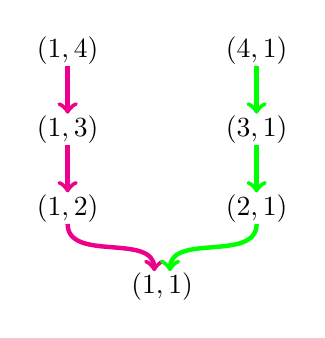
\begin{tikzpicture}[scale = 0.2]
    \node at (0,0) {$(1,1)$};

    \node at (-6,5) {$(1,2)$};
    \node at (6,5)  {$(2,1)$};

    \node at (-6,10) {$(1,3)$};
    \node at (6,10)  {$(3,1)$};

    \node at (-6,15) {$(1,4)$};
    \node at (6,15)  {$(4,1)$};

    \draw [->][color=magenta, ultra thick]
        (-6,14) to (-6,11);
    \draw [->][color=magenta, ultra thick]
        (-6,9) to (-6,6);
    \draw [->][out=-90,in=90, ultra thick] 
        [color=magenta](-6,4) to (-0.5,1);

    \draw [->][color=green, ultra thick]
        (6,14) to (6,11);
    \draw [->][color=green, ultra thick]
        (6,9) to (6,6);
    \draw [->][out=-90,in=90, ultra thick] 
        [color=green](6,4) to (0.5,1);

\end{tikzpicture}
\end{center}
        Chacun de ces posets comporte $\frac {1}{10} \binom{10}{3} = 12$
        éléments.
    \end{center}
\end{expl}

\begin{expl}[$a > b$ : Les posets de $\mathcal{LR}_{5,2}$ et
    $\mathcal{PF}_{5,2}$]
    ~\\
    \begin{center}
        \input{fig/fig19.tex}
        Pour plus de clarté, les flêches ont été simplifiées.
        Celles des deux plus hauts niveaux sont à comprendre ainsi :
        chaque flêche finit là ou il y a une croix de la même couleur.
        Il y a  $2^4 = 16$ éléments dans chacun de ces posets.
    \end{center}
\end{expl}


\begin{expl}[$a < b$ : Les posets de $\mathcal{LR}_{2,7}$ et
    $\mathcal{PF}_{2,7}$]
    ~\\
    \begin{center}
        \input{fig/fig20.tex}
        Il y a $7^1 = 7$ éléments dans chacun de ces posets.
    \end{center}
\end{expl}